\documentclass[UKenglish]{ifimaster}  %% ... or USenglish or norsk or nynorsk
\usepackage[latin1]{inputenc}        %% ... or utf8 or applemac
\usepackage[T1]{fontenc,url}
\urlstyle{sf}
\usepackage{babel,textcomp,csquotes,ifimasterforside,varioref,graphicx,caption}
\usepackage[section]{placeins}
\usepackage{amsmath}
\setcounter{secnumdepth}{3}

\usepackage{listings}
\usepackage{color}

\definecolor{mygreen}{rgb}{0,0.6,0}
\definecolor{mygray}{rgb}{0.5,0.5,0.5}
\definecolor{mymauve}{rgb}{0.58,0,0.82}

\lstset{ %
  backgroundcolor=\color{white},   % choose the background color; you must add \usepackage{color} or \usepackage{xcolor}
  basicstyle=\footnotesize,        % the size of the fonts that are used for the code
  breakatwhitespace=false,         % sets if automatic breaks should only happen at whitespace
  breaklines=true,                 % sets automatic line breaking
  captionpos=b,                    % sets the caption-position to bottom
  commentstyle=\color{mygreen},    % comment style
  deletekeywords={...},            % if you want to delete keywords from the given language
  escapeinside={\%*}{*)},          % if you want to add LaTeX within your code
  extendedchars=true,              % lets you use non-ASCII characters; for 8-bits encodings only, does not work with UTF-8
  frame=single,                    % adds a frame around the code
  keepspaces=true,                 % keeps spaces in text, useful for keeping indentation of code (possibly needs columns=flexible)
  keywordstyle=\color{blue},       % keyword style
  language=Java,                 % the language of the code
  morekeywords={*,...},            % if you want to add more keywords to the set
  numbers=left,                    % where to put the line-numbers; possible values are (none, left, right)
  numbersep=5pt,                   % how far the line-numbers are from the code
  rulecolor=\color{blue},         % if not set, the frame-color may be changed on line-breaks within not-black text (e.g. comments (green here))
  showspaces=false,                % show spaces everywhere adding particular underscores; it overrides 'showstringspaces'
  showstringspaces=false,          % underline spaces within strings only
  showtabs=false,                  % show tabs within strings adding particular underscores
  stepnumber=1,                    % the step between two line-numbers. If it's 1, each line will be numbered
  stringstyle=\color{mymauve},     % string literal style
  tabsize=2,                       % sets default tabsize to 2 spaces
  title=\lstname,                   % show the filename of files included with \lstinputlisting; also try caption instead of title
  numberstyle=\tiny,
}





\setlength{\parskip}{\baselineskip}%
\setlength{\parindent}{0pt}%


\title{Do Work in Progress (WIP) - Limit in Agile Software Development Matter?}        %% ... or whatever
\author{Truls Skeie}                      %% ... or whoever 
\usepackage[
    backend=biber,
    style=authoryear-icomp,
    sortlocale=de_DE,
    natbib=true,
    url=false, 
    doi=true,
    eprint=false
]{biblatex}
% !BIB TS-program = biber

\addbibresource{lib.bib}

\begin{document}
\ififorside{}
\frontmatter{}
\maketitle{}

\chapter*{Abstract}                   %% ... or Sammendrag or Samandrag

\tableofcontents{}
\listoffigures{}
\listoftables{}

\chapter*{Preface}                    %% ... or Forord

\mainmatter{}
\part{Introduction}                   %% ... or Innledning or Innleiing
\chapter{Background}  
\label{chap:Background}                %% ... or Bakgrunn
In this master thesis the main topics will contain analyzing of the gathered data from Software Innovation (SI) in order to see if WIP - limit it agile methods matters. SI is a Scandinavian software company that delivers Enterprise Content Management applications.From 2008 to 2013 SI gathered information about each task that was develop. The main reason SI gathered the data was to see if Kanban was more sufficient than Scrum for their use. For interested reader, the case study can be found in the article "Quantifying the Effect of Using Kanban versus Scrum: A Case Study" \parencite{Dag}. In this thesis the data will be used to determine if WIP-limit matters in agile methods.  

In the this chapter there will be a brief introduction of Scrum, Kanban, affiliated tools and to Software Innovation.

Research in the field of Work In Progress (WIP) and if WIP matters in software development, lacks proper research. But some similar research has been done, Giulio Concas and Hongyu Zhang  for instance has done research on the difference between limit WIP and unlimited WIP  \parencite{SMR:SMR1599} and David Anderson, Giulio Concas, Maria Ilaria Lunesu, and Michele Marchesi also highlighted the difference between limit WIP and unlimited process in the article 'Studying Lean-Kanban Approach Using Software Process Simulation' \parencite{DavidAnderson}

How to find the best WIP in software development (SD) for a given interval and context also lacks proper research, but in manufacture business some research has been done. Taho Yanga, Hsin-Pin Fub, Kuang-Yi Yanga stated that WIP could be defined as; ${WIP = cycle time * throughput \: rate}$ in manufacture business \parencite{Yang}.

\section{Kanban}
''We can define Kanban software process as a WIP limited pull system visualized by the Kanban board''  \parencite{DavidAnderson}.

Kanban system focus on;
\begin{itemize}
\item Continuous flow of work
\item	No fixed iterations or sprints
\item Work is delivered when it's done
\item Teams only work on few tasks at the time specified by the WIP limit
\item Make constant flow of released tasks
\end{itemize}
\parencite{DavidAnderson}.

Toyota production system introduced Kanban as a scheduling system for lean and just-in-time (JIT) production during late 1940's and early 1950's in order to catch up with the American car industry. The Kanban method combined with the lean approach was a success for Toyota. The success was noticed the software development industry among other. In the last ten years more and more software development companies have started to implement agile methods such as Scrum and Kanban \parencite{Conboy}, \parencite{ono1988toyota}. 

More and more software projects adapt to Kanban, and this is one of the reasons why this thesis will focuses on Kanban and WIP.
Kanban is one of the agile method in the wind these days, and is used with Lean Software development which is one of the fastest growing approaches in software development \parencite{DavidAnderson}
One of the most important people in Kanban software development, David Anderson  also referred to as ''father of Kanban in the software development industry''  \parencite{InfoQ:2013:May:Online} and author of the book "Kanban: Successful Evolutionary Change for Your Technology Business" once stated ''If you think that there was Capability Maturity Model Integration, there was Rational Unified Process, there was Extreme Programming and there was Scrum, Kanban is the next thing in that succession.''   \parencite{InfoQ} 

The Kanban method splits one big problem into many small pieces of problems. When the small pieces are defined by the team, the problems are put up on the Kanban-board to visualize the problems and see potential bottlenecks. When people started to understand Kanban, they easily discovered where the bottlenecks where \parencite{Shinkle}.


One of the main difference between Scrum and Kanban is estimation, in simulation of software maintenance process, with and without a work-in-process limit \parencite{SMR:SMR1599} estimation was defined to be the main source of waste. In their research, they find out, if they let the developers work with small tasks at time and not be interrupted, they will be more effective. The developers in this case was interrupted when they was assigned to estimate tasks. The research groups decided to implement Lean-Kanban, which includes minimizing waste, which meant estimation for this case. After implementing Lean-Kanban the teams increased the ability to perform work, lower the lead time and meet the production dates.

\section {Lean-Kanban}
The Lean approach was introduced between 1948 and 1975 in manufacturing work in Japan. It was designed to find and eliminate waste, so the manufacturing could deliver value to the costumer more efficiently. In 2003 Mary and Tom Poppendieck first introduced Lean thinking to software development, they published 'Principles of Lean Thinking' \parencite{Lean:2003}. Poppendieck stated that an important tool to manage work flow is the concept of pull-systems, which means tasks are put in production only when a costumer asks for it \parencite{Lean:2009}.
In the recent years, Kanban has been introduced more and more to software development, and is becoming one of the keys to Lean practice in the field \parencite{DavidAnderson}. 

\section {Scrum}
The Scrum framework is the source of much of the thinking behind principles and values of the Agile Manifesto. Values as "Individuals and interactions over processes and tools", "Working software over comprehensive documentation", "Customer collaboration over contract negotiation" and "Responding to change over following a plan" relates directly to Scrum. \parencite{Scrum}.

Scrum have three main roles, the Product Owner, the Scrum Master and the members of the development team. The Product owner in collaboration with the Scrum Master decides which work to be prioritized in the backlog. A backlog represents the tasks to be done in order to complete the project. The Scrum Master acts like a team leader and helps the team and organization to take best advantages of Scrum. The development team works on tasks specific for the sprint there in \parencite{Scrum}.

Sprint is a time-boxed interval over a given time. The Scrum framework suggests the duration of sprints to be from one to four weeks. Before each sprint, a sprint planning meeting is conducted, with all the team members attending.  A Sprint planning meeting is held so the team can discuss tasks from the backlog and come to an agreement of which tasks to be put in the minimal backlog.  \parencite{Scrum}.

In each sprint a minimal backlog is created so the developer knows which tasks to work on. The Product Owner and the team members discuss and decide which tasks from the backlog to be added to the minimal backlog. After the minimal backlog is full, the Product Owner and the team members discuss each task in order to get a better and a shared understanding of what is required in order to complete the task. One of the main principles in Scrum is that it requires that a new feature is ready for release after a sprint. The feature should be a visible part of the product in order to get feedback from end-users. So all the tasks in the minimal backlog combined should be a visible of the product.  \parencite{Scrum}.

\section {Kanban Board}
''The Kanban board makes it clear to all the team members the exact status of progress, blockages, bottlenecks and they also signal possible future issues to prepare for''\parencite{Joyce}.

The Kanban board is one of many important tools in Kanban. It's used to control the WIP, increase the information flow with visualization and spot bottlenecks \parencite{SMR:SMR1599}. A Kanban is board is illustrated in figure \ref{kanban_board}. Each column has an intuitive name in order to describe itself so the developers easily can track where each task is. In figure \ref{kanban_board} each column is named "Backlog", "In progress" and "Done".  Each column can have a WIP-limit to specify how many works in progress there are allowed in the column \parencite{Joyce}. In figure \ref{kanban_board} the WIP-limit is stated under the column name. The backlog columns have a WIP-limit of 4, In progress has 5 and obviously done doesn't have a WIP-limit.
\begin{figure}[ht!]
\centering
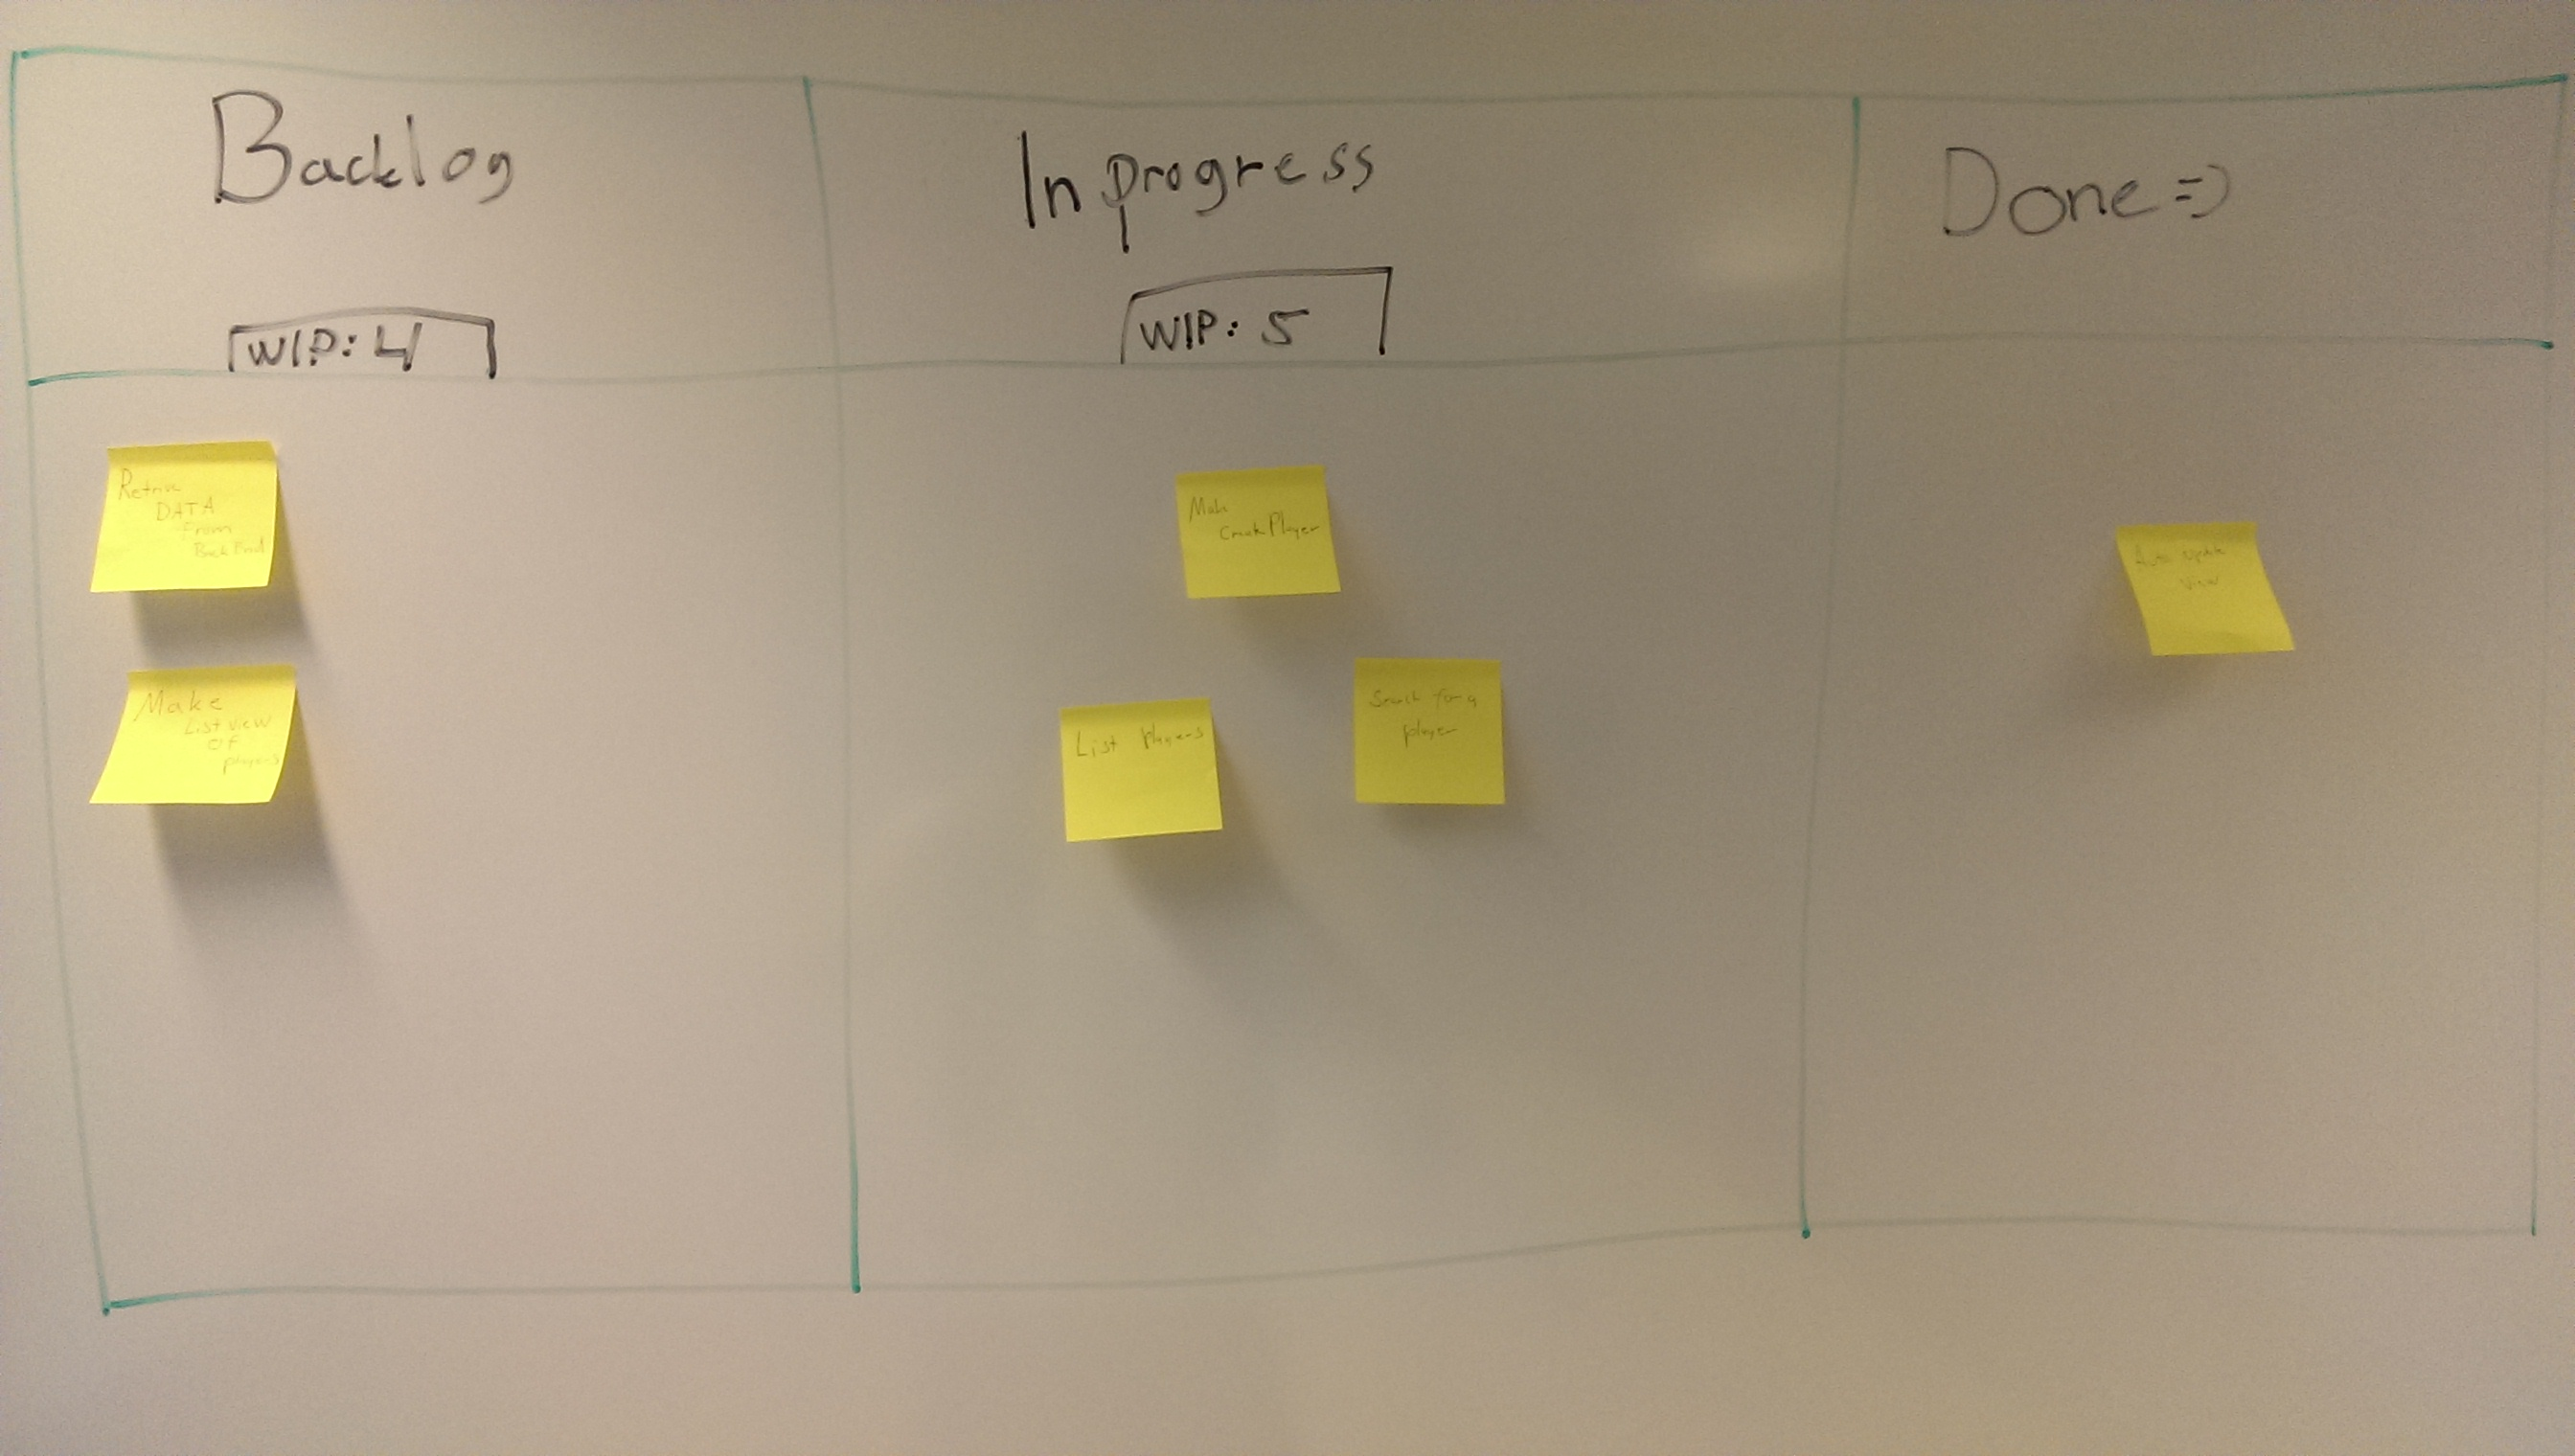
\includegraphics[width=90mm]{Picture/kanban_board.jpg}
\caption{Example of a Kanban board}
\label{kanban_board}
\end{figure}

\section {Lead time}
''Lead time is the total elapsed time from when a customer requests software to when the finished software is released to the customer'' \parencite{Joyce}.

The citation by Joyce above is close to definition of what lead time is. This definition could be useful for consultancy companies, but for SI, who is a big in-house development company with few releases each year this definition is unsuitable. Quantifying the effect of Using Kanban versus Scrum stated  two reason why this is unsuitable for SI: 

"First, the amount of time a work item remains in the backlog queue before it's put on the board is a function of priority, not whether the company uses Scrum, Kanban, or other development methods. Furthermore, companies that develop and sell products to many customers might propose new features themselves and put them on the backlog before any customers request them. Second, given a policy of two or three releases a year, the result of a work item isn't delivered to the customer immediately after it's finished'' \parencite{Dag}.

Lead time is an essential ingredient when you look for the optimal WIP. Often in project, lead time is split into pieces, so every task has its own lead-time; this gives the development teams the advantages to experiment with different WIP's in order to see the different lead-times and then measure which WIP that suits this project the best. 

\section{Just-In-Time}
"Just-In-Time is based on delivering only the necessary products, to the necessary time and the necessary quantity." \parencite{JIT}.

Just-In-Time was introduced 30 years ago by Toyota Motor in combination with Lean.  JIT has been developed to increase productivity through waste reduction and increasing the value added on the production processes. In one of the books by Mary and Tom Poppendieck the JIT principle is explained \parencite{Lean:2006}. To explain, illustrate and visualize the JIT principle Mary and Tom Poppendieck uses the picture \ref{JITE}  \parencite{JIT} \parencite{Lean:2006}.

\begin{figure}[ht!]
\centering
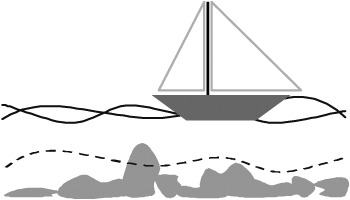
\includegraphics[width=90mm]{Picture/JIT.jpg}
\caption{JIT example}
\label{JITE} % JIT example
\end{figure}


In the picture \ref{JITE} the stream reflects the inventory.  Under the stream, there are rocks located in different sizes. The rocks illustrates waste and problems that can occur.  If the stream level is lowered, the rocks are more visualized. At this point you have to clear out rocks in order to make the boat continue it's journey, or it will crash into the rocks. After the rocks are cleaned out, you can lower the stream level again and continue until it's just pebbles left

If we lower the stream, problem and waste will become visible. But why do Lean want to lower inventory in order to make problems and waste occur? Because when problem and waste occurs, you are able to fix the problem and remove the waste. Fixing the problem and removing the waste can have several benefits such as, your process could be optimized and you are on step closer to have zero problems and zero waste.  \parencite{JIT} \parencite{Lean:2006}.


\section{Throughput}
''The output of a production process (machine, workstation, line plant) per unit time (e.g., parts per hour) is defined as the systems throughput or sometimes throughput rate'' \parencite{Adams}

The concept of throughput in order to measure how productive teams, people or companies is similar in both software development and manufacturing. On the other hand, in software development each task is more abstract, tasks can have different solutions depending on how the team or developer approaches the task and the tasks is usually only done once.

In manufacturing, each task usually has one solution and when the solution is found the physical item is mass produced.  Adam said "Throughput in plant, line or workstation, is defined as the average quantity of good  parts produced per unit time" \parencite{Adams}, which gives a good example of the relationship between tasks in manufacturing and software development. In manufacturing the part either fits its purpose (good) or not (defective), in software development a tasks can fit a purpose, but the purpose may be wrong.
 
In software development throughput is measured in number of finished delivered tasks per day, week, month, quarter or year. A key factor in successfully measuring throughput is to specify the size of each task. If the size is not specified   before, each tasks has to require almost the same amount of work.  
% As long as the software development task is bug free, it's delivered as non-defective but it may not fit the defined purpose by the end users. 

In software development throughput is measured in number of finished delivered tasks per day, week, month, quarter or year. A key factor in successfully measuring throughput is to specify the size of each task. If the size is not specified a developer x can have throughput of 1, but another developer y could have throughput of 3 and they still have done the same amount of work and this will give wrong results if the throughput is measured.  So its recommend to specify the amount of work for each task in advanced. 

\subsubsection{Example of throughput measurement}
This is a simple example to illustrate throughput and different task sizes. Team x had a throughput of eighteen tasks after the first quarter, twenty after the second, fifteen after the third and twelve after the last quarter and they used Scrum the first two quarters and Kanban the last two as illustrated by table \ref{tt}. It will look like team x benefits most from Scrum. But if the task during the Kanban time was twice the size of Scrum, Kanban would suite team x the best. In order to to get valid result from throughput measurement the size of tasks has to be agreed. 
\begin{table}[ht]
\begin{center}
    \begin{tabular}{| l | l | l | l |}
    \hline
    Quarter & Throughput &  Framework\\ \hline
    1 & 18 & Scrum\\ \hline
    2 & 20 & Scrum \\ \hline
    3 & 15 & Kanban\\ \hline
    4 & 12 & Kanban\\ \hline
    \end{tabular}
\caption{Throughput}
\label{tt} %% throughput table
\end{center}
\end{table}

\section{Chrun}
%%fylle inn?

\section{WIP}
''WIP-limits seem to be the worst understood part of the Kanban system. When used properly, it exposes bottlenecks and reduces lead time for individual work items. Used improperly, it can starve developers for work or result in too many people working on the same work items.'' \parencite{Shinkle}


WIP-limit is a tool in Kanban to reduce overhead by limit task-switching for each developer and visualize bottlenecks. One of the best way to explain WIP and the impact of WIP-limit is to use cars and roads as analogy. All roads have it maximum capacity width number of cars . When this limit is reached, traffic jam occurs and the throughput of cars decreases and lead time increases. The same can be said about software development teams, a software team has a maximum number of tasks they can perform, if the team is pushed over the maximum limit, the throughput of tasks decreases and lead time increases.

WIP-limit helps team to reduce overhead, decrease lead time and increase throughput \parencite {CONWIP}. But in order to get the best throughput and lead time, a software team needs to experiment with WIP in order to find their WIP-limit. When first implementing Kanban, Shinkle explains that the users don't care about the WIP, but rather the visibility of Kanban through the Kanban board. When the user get more experience with Kanban, they start to attempt the principles of WIP-limit \parencite{Shinkle}.

Shinkle defined novice and more experience kanban-users with a descriptive analogy \parencite{Shinkle}:
''Think about a typical person wanting to bake a cake. They go to the store, purchase a boxed cake mix, and follow the directions as described on the back of the box. They have little to no knowledge about how to alter the recipe nor do they have a desire to do so. Their goal is simply to bake a cake.''

''An advanced beginner understands how to apply some context to the instructions or rules on the back of the box. They can make minor adjustments for things like altitude, pan size, oven conditions, etc. They are still following the basic recipe, but can make minor adjustments likely based on previous experiences." According to Shinkle, principles like WIP-limit will be adopted when the user has some experience with Kanban. 

Setting the WIP-limit has a number of benefits according to Hopp, Spearman and Suri. They stated that it reduces flow times, reduces variation and improves quality \parencite{CONWIP}. However Srinivasan, Ebbing and Swearing said that setting the WIP is not easy. They suggest that WIP are just set, and then observe throughput, and adjust after that \parencite{Mandyam}. The principle of Kanban also says you should limit WIP. So what should the limit be? The principles of Kanban tells us to experiment \parencite{Kniberg}. Lean Software Management and the Impact of Kanban on Software Project Work suggest that WIP should be minimized as well. The study suggest to minimize WIP-limit to keep high quality \parencite{Ikonen} and to create continuous flow and bring problems to the surface \parencite{Joyce}. The conclusion of present study is to keep the WIP-limit low and experiment by slowing increase the WIP-limit until the throughput decreased and lead time increased, then you know that the previous WIP-limit was the perfect one.

Several people have their opinion on how to best measure the WIP, but most of them agree upon that's there is no clear rule of how to measure WIP in software development. Lukasz proposes to use The Effectiveness as an indicator measured at the end of each cycle. The effectiveness is a formula that takes the number of bugs found (ai) and the number of bugs found by external people (e.g. lawyers, accountants, coaches, consultants, translators, internal and external service providers ,etc.)(ei), and minus ai and ei, then divide the result by ai and multiply it by 100\%  as shown in \ref{WIPEQ} \parencite{Sienkiewicz}

\begin{equation} \label{WIPEQ}
Ei=\frac{ai-ei}{ai}*100\%
\end{equation}

\subsubsection{Benefits with WIP-limit according to research}
\begin{enumerate}
\item The tasks should be prioritized from high to low, in order to keep the best WIP. The article also states that high WIP will keep people task switching and not be able to fully concentrate on each work in progress \parencite{Ikonen}.
\item There's stated when using short-cycle times and Kanban board to limit WIP, the software development team's learning is increased' \parencite{Joyce}
\item The team in Lean Software Management study realized the where bottlenecks. So the team started to determine WIP by their constraints. The team quickly realized that they had fewer quality assurance/testing staff and business analysts than software developers. This reflected the bottlenecks and the constraints, so the team adjusted WIP to how much work they could handle; this gave the team more experience in dealing with WIP and increased productivity \parencite{Joyce}.
\end{enumerate}

As notice, there's no clear rule on how to deal with WIP and how to determine WIP, although WIP is a crucial tool in order to Kanban sufficient

\section {Limit WIP vs. Unlimited WIP}
Simulation of software maintenance process, with and without a work- in-process limit did a research on how the throughput and how developers experience WIP limit and unlimited WIP\parencite{SMR:SMR1599}.

One of the result from this paper was at the end of a simulation, the average of closed issued was 4145 when the WIP was limited and 3853 when the limit was not limited (about 7\% less). The paper concludes their finds like; developers are more focused on fixing few issues, because the number of issues they can work on is limited.  Because the limit of WIP, the developers are more likely to continue on the issue from the day before, rather than starting on another issue, this reduce overhead. When developers start on a new issue, they need to use time to familiarize themselves with the code and the issue. That could create unnecessary overhead if some developer already has done it, but that developer is now working on a another issue. The study also showed that limit WIP can improve throughput and work ef?ciency. \parencite{SMR:SMR1599}.

\section{Software Innovation(SI)}
Software Innovation is a Scandinavian software company. SI develops and delivers market-leading Enterprise Content Management applications that helps organizations improve and increase efficiency in document management, case handling and technical document control.

Software Innovation has approximately 300 employees, and has offices in Oslo, Copenhagen and Stockholm and a development center in Bangalore \parencite{SI}.


\part{The project}                    %% ... or ??
\chapter{Research Questions}
In this thesis the overall research question in this thesis is to study the effects of WIP limits in particular for SI. Some of the goals are:
\begin{itemize} 
\item See if the exist an optimal WIP-limit for a given context.
\item How to best find the optimal WIP-limit
\item Which various parameters taking in to account in order to optimize WIP. 
\end{itemize}
\chapter{Research Methods}
%%Skrive om weekends
In this section information about how my program will measure WIP, Items in backlog and throughput per date, per month, per quarter and per year will be explained. First off, there will be describe how the program do the measure in words, then the algorithm will be explained using algorithm in Pseudocode \parencite{jd}

The set from SI only contains dates when tasks was created, added to backlog, pulled from backlog or finished.  In order to measure average per month, quarter and year the program needs to know WIP and items in backlog for each day. In order to do so, the program will generate the remaining days.

Table \ref {dataset} show an excerpt from the dataset, as the reader may notice, the date 2008-10-09 is not in the set, so in this case, the program has to create 2008-10-09 and add it to the set

\begin{table}[ht]
\begin{center}
    \begin{tabular}{| l | l | l | l |}
    \hline
    Created Date\\ \hline
    2008-10-07\\ \hline
    2008-10-07 \\ \hline
    2008-10-07 \\ \hline
    2008-10-08\\ \hline
    2008-10-08\\ \hline
   2008-10-10\\ \hline
    \end{tabular}
\caption{Excerpt from the dataset}
\label{dataset} %% throughput table
\end{center}
\end{table}

The Date standard is specified as yyyy-mm-dd. \\
When I write iterate it means looping through the data with a for each-loop. \\
Quarter of a year is defined as January, February and March (Q1); April, May and June (Q2); July, August and September.\\ (Q3); and October, November and December (Q4) according to Investopedia \parencite{Quarter}

\section{Analyzed Data}
In this thesis the plan is to measure the data in one big step, where I measure all the teams and data in some given interval. I would also measure the data in small steps, when SI used Scrum, when SI was in the transforming phase and when they had changed to Kanban. Also I will measure WIP values for a given day, date, week, month, quarter and year. This will give me data to compare between teams in a specific interval.

I will reuse some data from the paper from Quantifying the Effect of Using Kanban vs. Scrum: A Case Study \parencite{Dag} Mainly I will look at churn and lead-time measured in the paper and compare them with WIP and throughput between teams. Hopefully the data measured will give me some sense of what WIP limit does for SI and which factors helping determine if WIP-limit matters in agile software development

Hopefully I would gather or get some other underlying data, so I will be able to compare my work, on the set from SI to the other data.

\section{Information about the dataset}
The set from SI contains almost thirty columns of different data. I will not examine every column in my thesis, but the columns I will use will be given a brief introduction to here.
\newpage
\subsection{The columns}
\begin{table}[ht]
\begin{center}
    \begin{tabular}{| l | p{5cm} |}
    \hline
     Column & Description\\ \hline
     Created Date & When a task is put in backlog \\ \hline
     Date From & When a given task is taken from the backlog\\ \hline
     Date to & When a task is done. Done is defined by SI to be ready for release. \\ \hline
    Lead Time & The amount of time elapsed from the date the task was created until the tasks has finished  \\ \hline
   Process Type &States the process used by the team which contains Kanban or Scrum \\
    \hline
    Team &States the team who has been working on the task.\\ \hline
    \end{tabular}
\caption{Information about the columns from the SI dataset}
\label{IC} %% information columns
\end{center}
\end{table}

\subsection {Algorithms for calculating WIP, backlog and throughput}
\begin{table}[ht]
\begin{center}
    \begin{tabular}{| l | l | p{5cm} |}
    \hline
    Variable &	Description	 & Columns from SI\\ \hline 
    Wip-Limit per day & \parbox[t]{5cm}{The number of items in progress on the given day} & Date From and Date To. \\ \hline
    Throughput	& Number of tasks finished on a given day & Date To \\ \hline
    Backlog & Number of items in backlog on a given day & Created Date and Date From\\ \hline
 Hashmap &\parbox[t]{7cm}{Hash table algorithm works by associating keys and their values in one-to-one mapping and storing them in a hashmap \parencite{Hashmap}} & \\ \hline
\end{tabular}
\caption{Description of variable and which columns from the SI set that is used to measure the variable}
\label{des} %% Description   
\end{center}
\end{table}

\begin{table}[ht]
\begin{center}
    \begin{tabular}{| l | p{5cm} |}
    \hline
     Key - Date  & Value - Integer\\ \hline
     2008-10-07 & 2   \\ \hline
     2008-10-08 & 0   \\ \hline
     2008-10-09 & 0   \\ \hline
     2008-10-10 & 2   \\ \hline
     2008-10-11 & 3   \\ \hline
     2008-10-12 & 0   \\ \hline
     2008-10-13 & 0   \\ \hline
     2008-10-14 & 2   \\ \hline
     2008-10-15 & 0   \\ \hline
     2008-10-16 & 0   \\ \hline
     2008-10-17 & 0   \\ \hline
     2008-10-18 & 0   \\ \hline
     2008-10-19 & 0   \\ \hline
     %%hva er dette til?
    \end{tabular}
\caption{skrive noe spennede}
\label{IC} %% information columns
\end{center}
\end{table}

\subsection {WIP-limit per day}
In order to describe the algorithm of measuring WIP limit per day, I will do it stepwise.  A detailed example on how the algorithm works is listed in the \ref{sec:Example}.

\subsection{Step 1: Gather all dates into a Hashmap}
\label{sub:stepOne}
First step of WIP measurement is adding every date in the date from column into a hashmap. Hashmaps contains key-value pairs, which will be respectively Date and Integer in this algorithm.  The date will contain the 'date from' column and the counter is number of occurrence of the date also known as WIP for that date. 

Pseudocode step 1:
 \begin{lstlisting}
for date IN date_from_column:
WIP = nr_of_date_ occurrence(date)
Hashmap.put(date, WIP)

nr_of_date_ occurrence(Date date) 
FOR d IN date_from_column DO
	if d EQUALS date DO
		nr_of_date_occurrence++
return nr_of_date_occurrence
 \end{lstlisting}
\subsection{Step 2: Gather the remaining days}
 \label{sub:stepTwo}
Since the 'date from' column do not contain all dates, the algorithm will create the remaining dates.  
In order to create the remaining dates, the program takes the first date and the last date from the hashmap created in previous (\ref{sub:stepOne}). Then the program checks if all the dates between the first date and the last date are in the hashmap. If the dates are not in the hashmap, the program will put the date into the hashmap.

Pseudocode step 2
 \begin{lstlisting}
First_date //points to the first date in the hashmap 
Last_date //points to the last date in the the hashmap 
Next_date //points to the next date
Next_date = First_date // Next_date assigned before iteration
while Next_date NOT EQUALS Last_Date
	New_date = Next_Date + 1 //Finds the date the next date
	AddToHashMap(New_date)
	Next_date = New_date

addToHashMap(Date d)
	if d NOT CONTAINS IN Hashmap
		Hashmap.put(date, 0) 
 \end{lstlisting}

\subsection{Step 3 Measure WIP}
Now that all the dates are in the Hashmap, WIP per day will be measured. Iteration through the Hashmap is necessary. Through the iteration each date and WIP is extracted from the Hashmap and the new WIP is measured based on how many tasks that has been finished, illustrated by the pseudo code.

Pseudocode step 3
The hashmap used in this pseudo code is the hashmap generated in section \ref{sub:stepTwo}.

\begin{lstlisting}
lastWIP =  0
CurrentWIP = 0
for date AND WIP IN Hashmap	
	CurrentWIP = WIP 
	Nr_of_finishedDates = Occurrence_of_date(date)  
	WIP_measured = CurrentWIP - Nr_of_finishedDates + lastWIP
	newHashMap.put(date, WIP_measured)
	currentWIP = WIP_measured 

Occurrence_of_date(Date date)
	for d in The Date To column
		if date AFTER d DO
			Nr_of_dates_to_decrement++
Return Nr_of_dates_to_decrement 
 \end{lstlisting}

\subsection{Example}
\label{sec:Example}
Figure \ref{wip_timeline}  shows tasks id in the y-axis and dates in the x-axis. The green line indicates the duration of the task. This table indicates how many tasks in progress (WIP). On 2008-10-12, tasks 3, 5 and 6 are in progress, which means WIP is three for 2008-10-12.  
\begin{figure}[ht!]
\centering
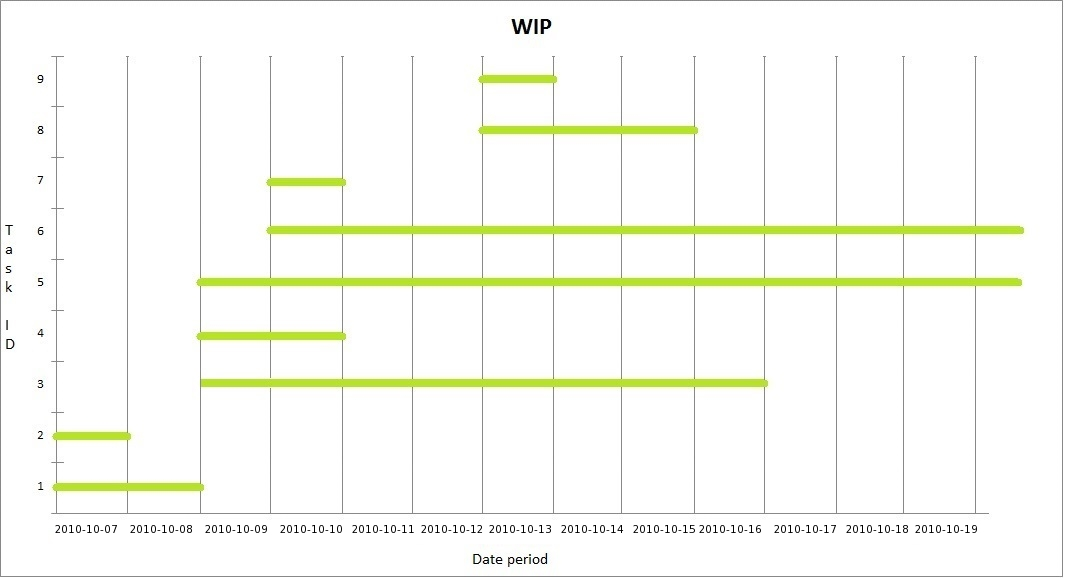
\includegraphics[width=150mm]{Picture/wip_example.jpg}
\caption{Illustrating a WIP timeline}
\label{wip_timeline}
\end{figure}

\begin{table}[ht]
\begin{center}
    \begin{tabular}{| l | l | p{5cm} |}
    \hline
   Task ID &   Date From  & Date To\\ \hline
     1 & 2008-10-07 & 2008-10-08   \\ \hline
     2 & 2008-10-07 & 2008-10-07   \\ \hline
     3 & 2008-10-09 & 2008-10-16   \\ \hline
     4 & 2008-10-09 & 2008-10-10   \\ \hline
     5 & 2008-10-09 & 2008-11-04   \\ \hline
     6 & 2008-10-10 & 2008-10-05   \\ \hline
     7 & 2008-10-10 & 2008-10-10   \\ \hline
     8 & 2008-10-13 & 2008-10-15   \\ \hline
     9 & 2008-10-13 & 2008-10-15   \\ \hline
    \end{tabular}
\caption{Showing Task ID, Date From and Date to}
\label{wt:2} %%  wip table 2
\end{center}
\end{table}

\begin{center}
    \begin{tabular}{| l | l | p{5cm} |}
    \hline
   Task ID &   Date From  & Date To\\ \hline
     10 & 2008-10-07 & 10\\ \hline
     11 & 2008-10-07 &  43\\ \hline
     12 & 2008-10-09 & 65   \\ \hline
     13 & 2008-10-09 & 30   \\ \hline
     14 & 2008-10-09 & 25   \\ \hline
     15 & 2008-10-10 & 85   \\ \hline
     16 & 2008-10-10 & 57   \\ \hline
     17 & 2008-10-13 & 24   \\ \hline
     %18 & 2008-10-13 & ?  \\ \hline
    \end{tabular}
    \captionof{table}{Showing Task ID, Date From and Date to}

\label{wt:3} %%  wip table 3
\end{center}

In the example dates from figure \ref{wip_timeline} and from table \ref{wt:2} (skal gel ha med table tre her go) will be used to illustrate how the algorithm measure WIP

\subsubsection{First step}
\label{subsubsec:ft}
First the algorithm will do a look-up on the date 2008-10-07 referred with task ID one and two in WIP Table 2 and measure the current WIP counter, which is two, because its two tasks in progress on this date. Then, the program will put the date and the current WIP into a hashmap. 
Next, the algorithm will see if any task was done in the last period, since task one and two is the two first tasks to be measured in this example, there's no task finished in the period and there's no WIP from other tasks, so the current WIP at 2008-10-07 is two illustrated by figure \ref{wip_timeline}. 
\subsubsection{Second step}
The program will do a look-up on the date 2008-10-09 referred with task ID three, four and five in table \ref{wt:2}  and measure the current WIP for this date, which is three. Then, the program will put the date and the current WIP into a hashmap.
Next, the program will see that two tasks were done in the period of 2008-10-07 to 2008-10-09. So the program will measure that three new tasks were started at 2008-10-09, two where finished and the WIP from last date measure where two, so the calculation of WIP at 2008-10-09 is 3-2+2, which gives a WIP of three on 2008-10-09 illustrated by figure \ref{wip_timeline}. 

\subsubsection{Third step}
The program will do a look-up on the date 2008-10-10 referred with task ID six and seven in table \ref{wt:2}  and measure the current WIP for this date, which is two. Then, the program will put the date and the current WIP into a hashmap.
Next, the program will see that no task where done in the period 2008-10-09 to 2008-10-10 and the currently WIP is three, so this gives a new WIP of 5 illustrated by figure \ref{wip_timeline}. 

\subsubsection{Fourth step}
The program will do a look-up on the date 2008-10-13 referred with task ID eight and nine in table \ref{wt:2}  and measure the current WIP for this date, which is two. Then, the program will put the date and the current WIP into a hashmap. 
Next, the program will look at the period between 2008-10-10 and 2008-10-13, and see that task four and seven was done in this period. The WIP at 2008-10-13 will be $2-2+5 = 5$ as illustrated by figure \ref{wip_timeline}. 
As illustrated by the example, WIPs are not decrement until the finished date is passed, even though the task is done on the date, it's also worked on the same date, therefore I have chosen to decrement the WIP after each date is passed.

\subsection {Bug}
\label{Bug}
Each task in the data set is label as either feature or bug as shown in figure \ref{bugsT}. When the program reads in the data file, each task label as bug are saved in a data structure as shown in listing \ref{findBug}.

\begin{table}[ht]
\begin{center}
    \begin{tabular}{| l | l | p{5cm} |}
    \hline
    Task ID & Type \\ \hline
57970 &	Bug\\ \hline
57971&	Bug\\ \hline
57972&	Bug\\ \hline
57973&	Bug\\ \hline
57974&	Feature\\ \hline
57975&	Feature\\ \hline
57976&	Feature\\ \hline
57977&	Feature\\ \hline
57978&	Feature\\ \hline
    \end{tabular}
\caption{Example of how tasks are labeled}
\label{bugsT} %%  bugs table
\end{center}
\end{table}
\newpage

\begin{lstlisting}[caption=Pseudocode example of how bugs are found, label=findBug]
void findBug()
	while inputFile != EOF
		newLine = readLine()
		if newLine.Type EQUALS 'Bug'
			B = New Bug()
			B.startDate = newLine.startDate
			B.process = newLine.process
			B.team = newLine.team 
			AddNewBug(B)
 \end{lstlisting}

\subsection{Add Bug}
\label{addBugS}
When adding a new bug to the data structure, each bug is gathered into a data structure based on which team the bug belongs to, as the tests in lines 2, 7, 12 and 17 of the listing \ref{addBug} shows. After the right team is found the program tries to add the bug to the corresponding data structure as illustrated in lines 3, 8, 13 and 18. If the date of newly arrived bug already contains in the data structure, a counter representing the date is incremented and the new bug is discarded as shown the method dateExists in lines 26 to 32. 

Since the program knows which team the new bug belongs to (after the checks on line 3, 8, 13 and 18) a counter can represent each bug. In our analyze the only important for us is to know how many bugs there are on a given date and which team it belongs to.  
\newpage
\begin{lstlisting}[caption=Pseudocode example of how bugs are added, label=addBug]
void addBug(Bug b)
	if b.team EQUALS "360"
		if dateExists(b.date, 360.dataStructure) EQUALS false
			// if date don't exists, then add the bug
			360.dataStructure.add(b)
			
	if b.team EQUALS "Neon"
		if dateExists(b.date, Neon.dataStructure) EQUALS false
			// if date don't exists, then add the bug
			Neon.dataStructure.add(b)
			
	if b.team EQUALS "Frontend"
		if dateExists(b.date, Frontend.dataStructure) EQUALS false 
			// if date don't exists, then add the bug
			Frontend.dataStructure.add(b)
			
	if b.team EQUALS "Krypton"
		if dateExists(b.date, Krypton.dataStructure) EQUALS false
			// if date don't exists, then add the bug
			Krypton.dataStructure.add(b)
		
void dateExists(Date d, DataStructure structure)
	for Bug b in structure
		if b.date EQUALS d
			b.counter++
			return true
	
return false	
 \end{lstlisting}
 
 \subsection{Throughput}
Finding the throughput per day is quite similar to how bugs are found (described in section \ref{Bug}).  When reading in the data set a new throughput object is created for each line in the set.  Then all throughput objects are sorted based on team association. When all throughput objects are sorted, the program measure throughput. The throughput measurement is similar to the dateExists method (lines 26 to 32) in the listing \ref{addBug} stated in section \ref{addBugS}. 

\newpage
The dateExists method starts of with a test, the same test is done for throughput, if the date of the throughput object is in the data structure the corresponding counter is incremented.  If the date is not in the data structure, the new throughput object is added to the data structure. An excerpt of the code is listed in \ref{throughputCode} 

\begin{lstlisting}[caption=Pseudocode example of how throughput is measured, label=throughputCode]

void dateExists(Date d, DataStructure structure)
	for Throughput t in structure
		if t.date EQUALS d
			t.counter++
			return true
			
return false	
\end{lstlisting}
 
\section{Analyze the created data}
From the data created i will analyze them using SPSS.
\subsection{SPSS}
IBM SPSS Statistics is a software product for managing data and calculating a wide variety of statistics. SPSS is built around the SPSS programming language. 

\subsection{Analyzed data per quarter}

\begin{figure}[!htbp]
\centering
%%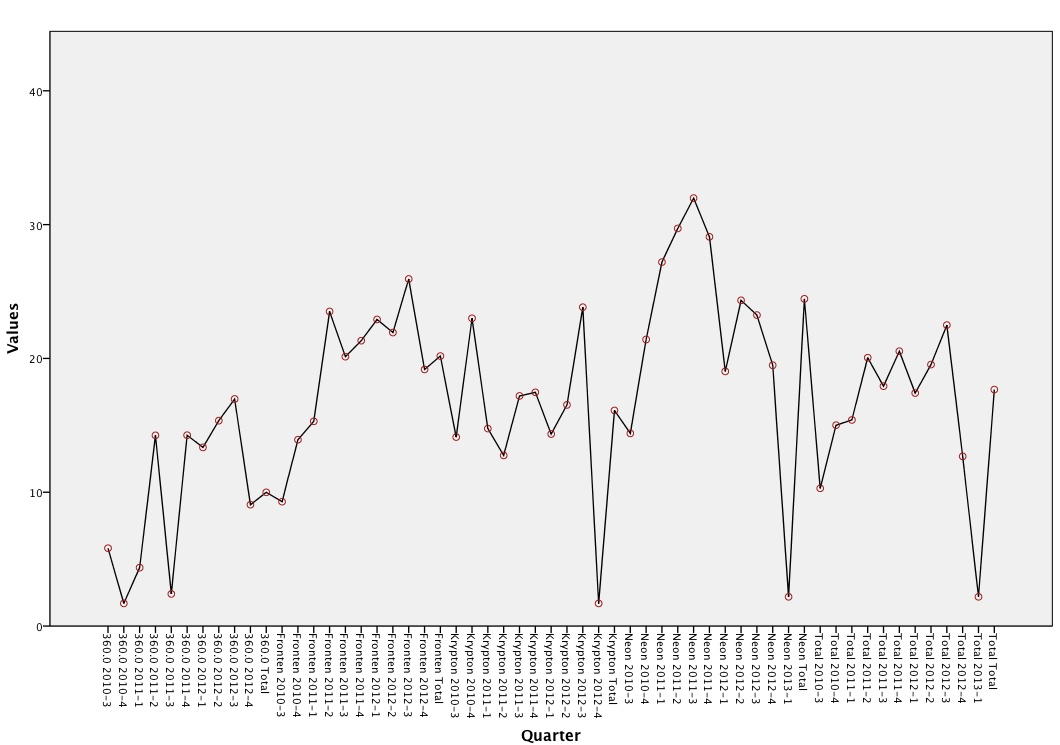
\includegraphics[scale=0.5]{Picture/All_WIP.jpg}
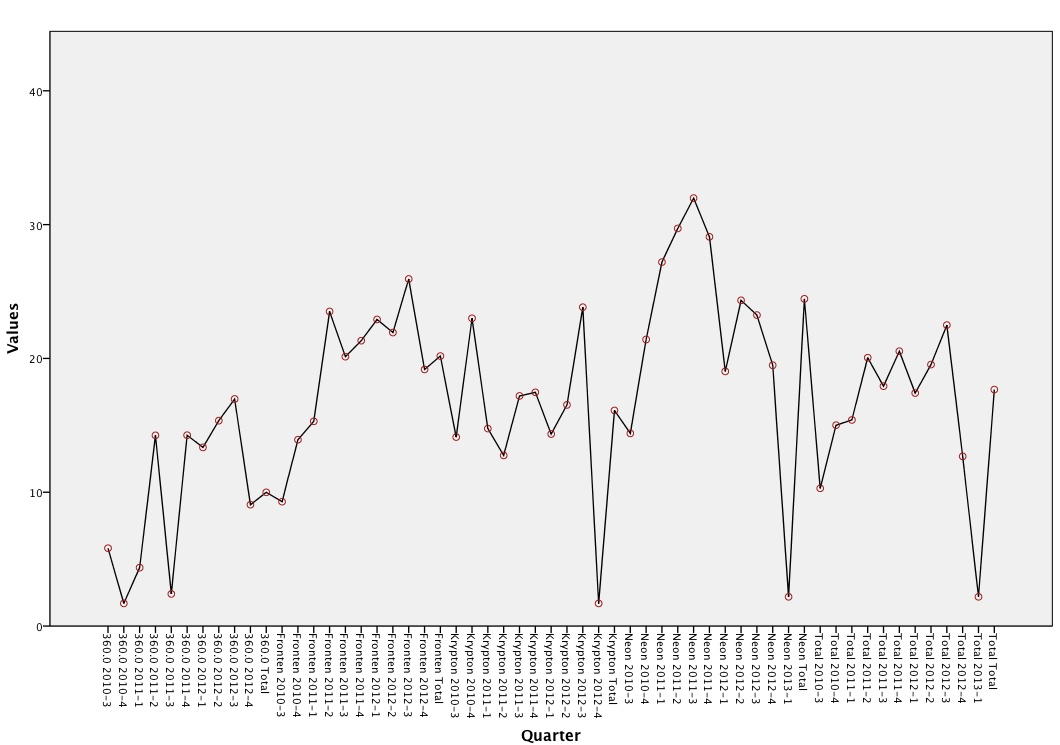
\includegraphics[width=\textwidth,height=\textheight,keepaspectratio]{Picture/All_WIP.jpg}
\caption{WIP for 360 per quarter}
\label{W360pq} %% 360 per quarter
\end{figure}



\chapter{Planning the project}        %% ... or ??


\part{Conclusion}                     %% ... or Konklusjon

\chapter{Results}                     %% ... or ??


\backmatter{}
\printbibliography
\end{document}
